%コンパイル方法: opt+cmd+b → opt+cmd+v
\RequirePackage{plautopatch}

\documentclass[a4paper, 9pt]{ltjsarticle}


% マージン設定
\usepackage[top=20mm, bottom=20mm, left=20mm, right=20mm]{geometry}

% LuaLaTeX用日本語対応パッケージ
\usepackage{luatexja}
\usepackage{luatexja-fontspec}

% 必要なパッケージ
\usepackage{fontspec}
\usepackage{titlesec}
\usepackage{graphicx}
\usepackage{amsmath}
\usepackage{amssymb}
\usepackage[hidelinks]{hyperref}
\usepackage[english, japanese]{babel}
\usepackage{multicol} % 二段組用パッケージ
\usepackage{indentfirst}
\usepackage{tikz} % カスタム点線用
\usepackage{authblk} % 著者・所属パッケージ
\usepackage{here}
\usepackage{caption}
\usepackage{bookmark}
\usepackage{array}
\usepackage{booktabs}
\usepackage{diagbox} % 斜線を入れるためのパッケージ


% \setmainfont[Ligatures=TeX]{Times New Roman}
% \setmainjfont[BoldFont=MS Gothic]{MS Mincho}

\renewcommand{\baselinestretch}{0.95}
\renewcommand{\labelenumi}{(\arabic{enumi})}

% セクション見出しのカスタマイズ
\titleformat{\section}
  {\fontsize{10pt}{10pt}}
  {\thesection.}
  {1em}{}

\titleformat{\subsection}
  {\fontsize{10pt}{10pt}}
  {\thesubsection}
  {1em}{}

\titleformat{\subsubsection}
  {\fontsize{10pt}{10pt}}
  {\thesubsubsection}
  {1em}{}

  \setlength{\parindent}{1em}
% \setlength{\belowcaptionskip}{1em} % キャプション下の余白を -10pt に設定


%section前に余白を作る
\titlespacing*{\section}{0em}{1em}{0em}
\titlespacing*{\subsection}{0em}{1em}{0em}
\titlespacing*{\subsubsection}{0em}{1em}{0em}

\pagestyle{empty}


\begin{document}

\setlength{\columnsep}{7.5mm}

\twocolumn[
    \begin{center}
        {\vspace{-1em}}

        {\fontsize{15pt}{15pt}\selectfont{災害時を想定したアドホックネットワーク構築手法の検討}}

        {\vspace{1.5em}}

        {\fontsize{13pt}{13pt}\selectfont{A study of ad hoc network construction methods for disaster scenarios}}
    \end{center}



    \begin{flushright}
      {\fontsize{11pt}{11pt}\selectfont{T5-17 末廣隼人\\}}
      {\fontsize{11pt}{11pt}\selectfont{指導教員 髙﨑和之}}
    \end{flushright}

    \vspace{1em}

    \thispagestyle{empty}
]

\section{はじめに} \label{label:first}
% 昨年、1月1日に石川県能登半島にて発生した最大震度7の大地震など日本では多くの自然災害が発生しており、その中で一番恐れられている災害として地震がよくあげられる。
% また最近では、南海トラフ地震が30年以内に来ると言われており、その時の被災状況として静岡県から宮崎県にかけての一部では震度7、
% その隣接する周辺の広い地域では震度6強から6弱の強い揺れと想定\cite{南海トラフ地震}されている。
% 現代ではスマートフォン等から情報を取得しているが、先ほどのような大地震が発生したとき、ネットワークへのアクセス集中や電波基地局の倒壊によりネットワーク障害が生じてしまい、
% 救助を要請する方達の声が届かなくなってしまう。このような状況の解決手段として、一時的なネットワークを作成することでその地域内限定ではあるが情報共有が可能になる
% アドホックネットワークやメッシュネットワークを利用した研究が行われている。\par
% 本研究では、突然襲ってくる地震に対して大勢の中でも経路が複雑化しないようノードの密度で接続数を変化させるようにし、どのノード密度のとき広範囲にネットワークを広げられるかを
% シミュレーションにより検討を行った。


% 自然災害、特に地震発生時に基地局の倒壊やネットワーク障害が生じたときに、
% その間に助けを求める人達の不安を少しでも拭うために一時的なネットワーク、
% アドホックネットワークの構築を行い少しでも多くの情報を共有できることを目的として研究を行った。\\
% 具体的には、被災エリアの中心に主となるノードを設置、その周りに携帯端末が保有するBluetoothなどでアドホックネットワークの構築おこうなう。
% このとき、全ての端末をアドホックに使用してしまうと、ルーティングが煩雑distribution化してしまうしまうため、
% アルゴリズムでメインとして使用する端末と接続が切れてしまった時の補助端末に分ける。その方法を第3章で述べる。

% 日本では多くの自然災害が発生しており、自然災害の中で一番恐れらている災害が地震であった。
% 昨年の石川県能登半島で発生した大地震では多くの死傷者がでてしまい、甚大な被害を被った。
% この災害では特に高齢者の人口が多く占めており、迅速な避難が難しかったり、

% \section{研究背景}

\section{理論} \label{label:theory}
\subsection{アドホックネットワーク} \label{sublabel:about ad-hoc network}
アドホックネットワークとは、中央の管理者やルータ、アクセスポイント等の既存のインフラストラクチャを介さずに、端末(以降ノードという)同士が直接通信を行う一時的なネットワークのことである。
遠くのノードと通信を行う場合、隣接する他ノードを中継機として利用し、バケツリレーのようにデータを送信するマルチホップ通信技術を用いる。%
\\ \indent 本研究では、低コスト、低消費電力でスマートフォンに内蔵されているBluetoothを用いたアドホックネットワークを想定し、
より消費電力が少ないBluetooth Low Energy(BLE)の接続目安距離である30mを最大通信距離としてシミュレーションを行った。

\subsection{ルーティング制御方法} \label{sublabel:routing control}
各ノードが通信を行う際のルーティング方式には大きく分けてリアクティブ型、プロアクティブ型、ハイブリッド型の3種類がある。
各方式の特徴を次に示す。本研究では、ハイブリッド型を参考に経路生成手法の検討を行なった。
\begin{enumerate}
  \item \label{reactive} リアクティブ型 \par  
  \indent 通信要求が発生した時に近くのノードとその場でデータのやり取りを行い経路を作成する。
  通信開始までに遅延が生じるが経路情報維持のための通信が不要なため通信頻度の低い環境では消費電力が少なく長時間使用できる。
  代表的なプロトコルとしてAODVやDSRなどがある。

  \item \label{proactive} プロアクティブ型 \par
  \indent 近くのノード間で自身の情報をやりとし経路をあらかじめ作成する。あらかじめ経路が作成されるため、通信開始までの遅延が短い。  
  しかし、定期的にデータのやり取りを行うため消費電力が多い。代表的なプロトコルとしてOLSRやTBRPFなどがある。

  \item ハイブリッド型 \par
  \indent (\ref{reactive})、(\ref{proactive}) の二つを組み合わせたルーティング方式である。代表的なプロトコルとしてはZRPなどがある。
\end{enumerate}

\section{提案手法} \label{label:proposed method}
\subsection{想定環境} \label{sublabel:expected environment}
経路生成のシミュレーションにあたりノードの密度は日本の人口密度にスマートフォンの所有率88.6\%\cite{スマホ保有率}を乗じた数とした。%
人口密度が高い地域として埼玉県、低い地域として福島県2つの地域に対してシミュレーションを行った。
また、人口密度が低い地域ではノード同士の間隔が大きくなってしまうため、電柱にBLE機能とを有した低コストの機器(以降電柱ノードという)を設置した2つの場合についてのシミュレーションを行った。\par
ノードは1km四方の範囲内に配置し、その中で中心に近いノードをインターネットにつながるゲートウェイ(以降スタートノードという)として、そこから一番遠いものをターゲットノードとして経路を探索した。\par
% 電柱の設置間隔は約30m\textasciitilde 50m \cite{電柱設置間隔}であるが、人口密度により増減がバラバラになってしまう。
% そのため、今回はそれぞれの地域の人口密度に電柱一本がカバーする人数[人/本]で割った数を電柱の数とした。
以下にそれぞれの地域に対応した数値を載せる。

\begin{table}[h]
  \centering
  \caption{2024年10月1日現在の自治体構成}
  \begin{tabular}{c|cc}
    \specialrule{1.5pt}{0pt}{0pt} % 上端の太線(1.5pt)
      県名 & 埼玉県 & 福島県 \\
      \hline
      人口密度 [人/$\mathrm{km}^2$] \cite{人口密度} & 1930 & 126 \\
      ノードの数 [個] & 1710 & 112 \\
      \specialrule{1.5pt}{0pt}{0pt} % 上端の太線(1.5pt)
  \end{tabular}
\end{table}

\subsection{人口密度が高い地域の場合} \label{sublabel:high population density}
% 理由
人口密度が高い地域では全てのノードが1つのアドホックネットワークに接続してしまうと経路の複雑化や経路の冗長化により、通信速度や通信品質の低下が発生してしまう。
これらを解決するために、周辺ノードの密度を用いて接続ノードを制限し経路の単純化を行った。ノードの接続条件を次のように定めた。 \par

\begin{itemize}
  \item 上流ノードが下流ノードに対してhelloメッセージと自身のMACアドレスをフラッディングする。
  \item 受信した下流ノードはreplyメッセージとMACアドレス上流ノードに返す。但し、他ノードと接続済みの下流ノードは上流ノードのhelloメッセージを無視する。
  \item 上流ノードはhelloメッセージの返信数で下流ノードの数を認識する。
  \item 下流ノード数が$X$より大きいなら下流ノードの中からランダムで1つ選択し、そうでないならランダムで2つ、下流ノード数が2以下ならそのノードと接続する。
\end{itemize}

この$X$にはノード密度の閾値が入り、それぞれ2\textasciitilde7の場合でシミュレーションを行った。

\subsection{前述の手法について} \label{sublabel:high population density methods}
人口密度が高い埼玉県の条件を用いた場合のシミュレーション結果を次に述べる。 \par
\begin{enumerate}
  \item シミュレーション実行結果 \par
  \indent ノード密度が5の場合のシミュレーションの実行結果を図\ref{fig:1}に示した。グラフの色について説明する。
  赤点は中心に近いものがスタートノード、もう1つの赤点はターゲットノード、青点は接続可能ノード、
  オレンジ点は接続不可能ノード、薄青で塗られている部分は接続可能面積である。接続されていない青点ノードがいくつかあるが、
  これは経路生成時に余ったノードであるため、万が一近くのノードが消滅した時の代替として使用できるため青点になっている。
  \begin{figure}[ht]
    \centering
    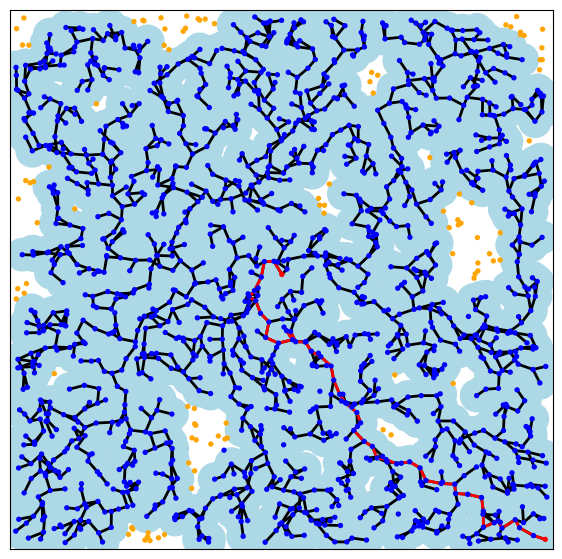
\includegraphics[width=65mm]{シミュレーションの様子.png}
    \caption{ノード密度の閾値が5のシミュレーション実行結果}
    \label{fig:1}
  \end{figure}

  \item 最適なノード密度について \par
  \indent 各ノード密度の閾値で10回ずつシミュレーションを行い、接続可能ノードをノードの総数で割った接続可能ノード割合の平均値を図\ref{fig:2}
  に示した。この図より、閾値が5のとき接続可能ノード割合が75.9\%で一番高くなった。 \par
  \begin{figure}[ht] % [h]は「ここに表示」の意味
    \centering
    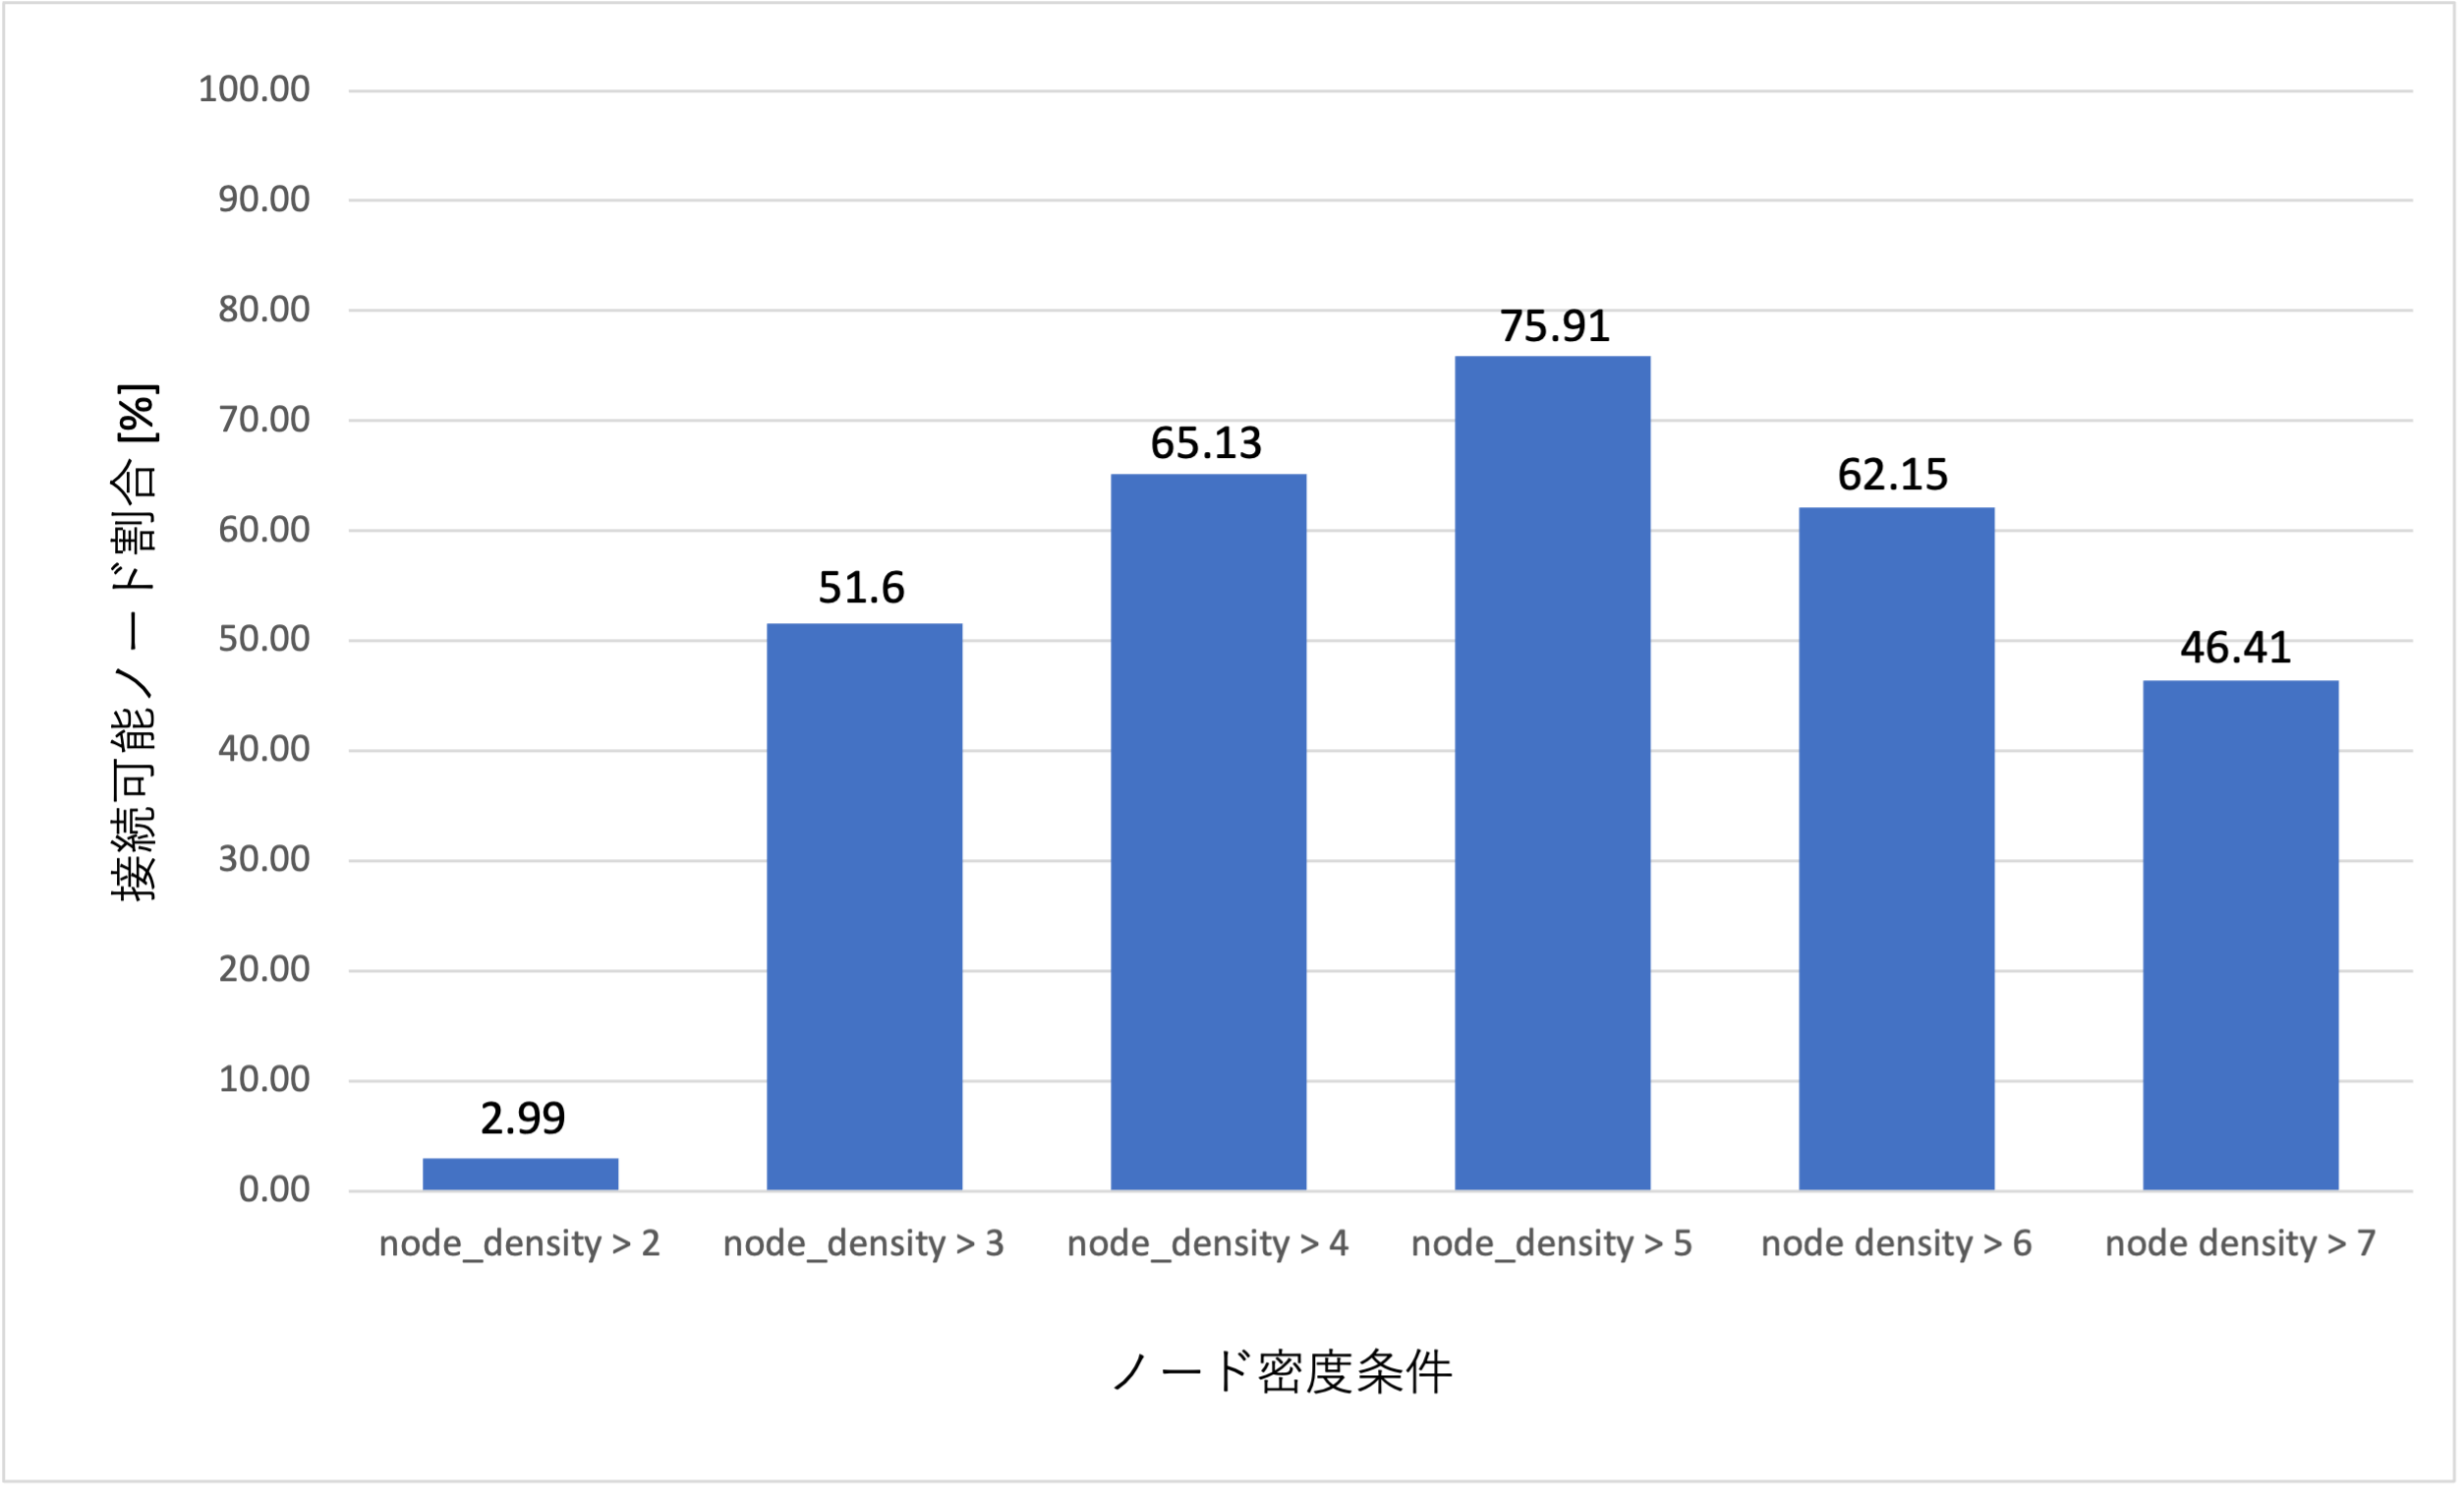
\includegraphics[width=80mm]{提案1の結果.png}
    \caption{人口密度が高い地域の場合}
    \label{fig:2} % 参照用のラベル
  \end{figure}

  \item 人口密度が低い地域の場合 \par
  \indent 紙面の都合上、人口密度が低い地域については結果だけ述べさせていただく。どのノード密度の条件でも接続可能ノード割合は0\textasciitilde5\%の間であった。
  これは、ノードの間隔が大きく偶然近くにいたとしてもその先にノードが存在しないため、ネットワークを広げることができないと考えられる。
\end{enumerate}

\subsection{人口密度が低い地域の場合} \label{sublabel:low population density}
\ref{sublabel:high population density}では人口密度が高い地域でのみ使用できたが、人口密度が低い地域ではノード間隔が広すぎるためネットワークを広げることができなかった。
そこで、電柱を利用することでノードの補完を行った。また、使用するノード密度の閾値は提案手法-1で判明した5を用いる。\par
電柱ノードの生成、接続条件を次のように定めた。

\begin{itemize}
  \item 人口密度が高い地域では電柱を30m間隔、低い地域では50m間隔で生成する。
  \item 電柱ノード同士は指向性の強い電波でやり取りを行う。電柱ノードとノードの接続には提案手法-1と同様の条件で行う。
\end{itemize}

\subsection{前述の手法について} \label{sublabel:low population density methods}
人口密度が低い福島県の条件を用いた場合のシミュレーション結果を次に述べる。

\begin{enumerate}
  \item aa
\end{enumerate}

\section{考察} \label{label:consideration}
% 提案手法-1のシミュレーション結果より、周辺ノードの密度が4\textasciitilde6のとき経路生成が多く行われることがわかった。
% しかし、図\ref{fig:2}のようにノードの位置が均一になっていないため密から疎の地域へ通信を拡大することができなかった。
% そのため、今後の課題として電柱や街灯等の動かずかつ、一定間隔に設置されているシンボルにノードを設置することでノードの総数を
% 増やす必要があると考えられる。

\section{まとめ} \label{label:conclusion}
% 本研究では、災害時を想定したアドホックネットワーク構築する際、多量のノードにより複雑化してしまう経路を
% 下流ノードの接続状況と周辺のノード密度を考慮することにより簡単な経路探索する手法を検討した。
% その結果、周辺ノードの密度が4\textasciitilde6であるとき広範囲なネットワークを生成することができた。
% また、ループが発生しないため通信品質も保つことができると考えられる。しかし、スタートノード周辺のノードの負荷が大きくなってしまうため、
% 複数のスタートノードを用意し、負荷の分散を行う必要があると考えられる。\par
% 今回のシミュレーションでは、アドホックネットワークの技術的課題について触れていないため実際の環境では異なる結果が出ると考えられるため、
% 今後は実環境で実験を行いそれを元にシミュレーションを改良していきたいと考えている。

\begin{thebibliography}{9}
  \bibitem{南海トラフ地震} \url{https://www.jma.go.jp/jma/kishou/know/jishin/nteq/assumption.html}, 国土交通省 気象庁, "南海トラフ地震で想定される震度や津波の高さ"
  \bibitem{スマホ保有率} \url{https://www.soumu.go.jp/johotsusintokei/whitepaper/ja/r04/html/nd238110.html}, 総務省, "通信利用動向調査」"
  \bibitem{電柱設置間隔} \url{https://www.tepco.co.jp/pg/company/press-information/press/2019/pdf/190808j0101.pdf}, 東京電力, "全国の「位置情報データ」の代理店販売の概要"
  \bibitem{人口密度} \url{https://uub.jp/rnk/p\_j.html}, 都道府県市区町村, "都道府県 人口・面積・人口密度ランキング"
\end{thebibliography}

\end{document}
